Dans le but de pousser notre implémentation de la LBM un peu plus loin, nous avons simulée le flux autour d'une aile d'avion, le but était d'obtenir nos premiers écoulements dépendant du temps, voici en figure \ref{fig:VK} un des résultat que nous avons obtenu.

\begin{figure}[hbtp]
  \centering
  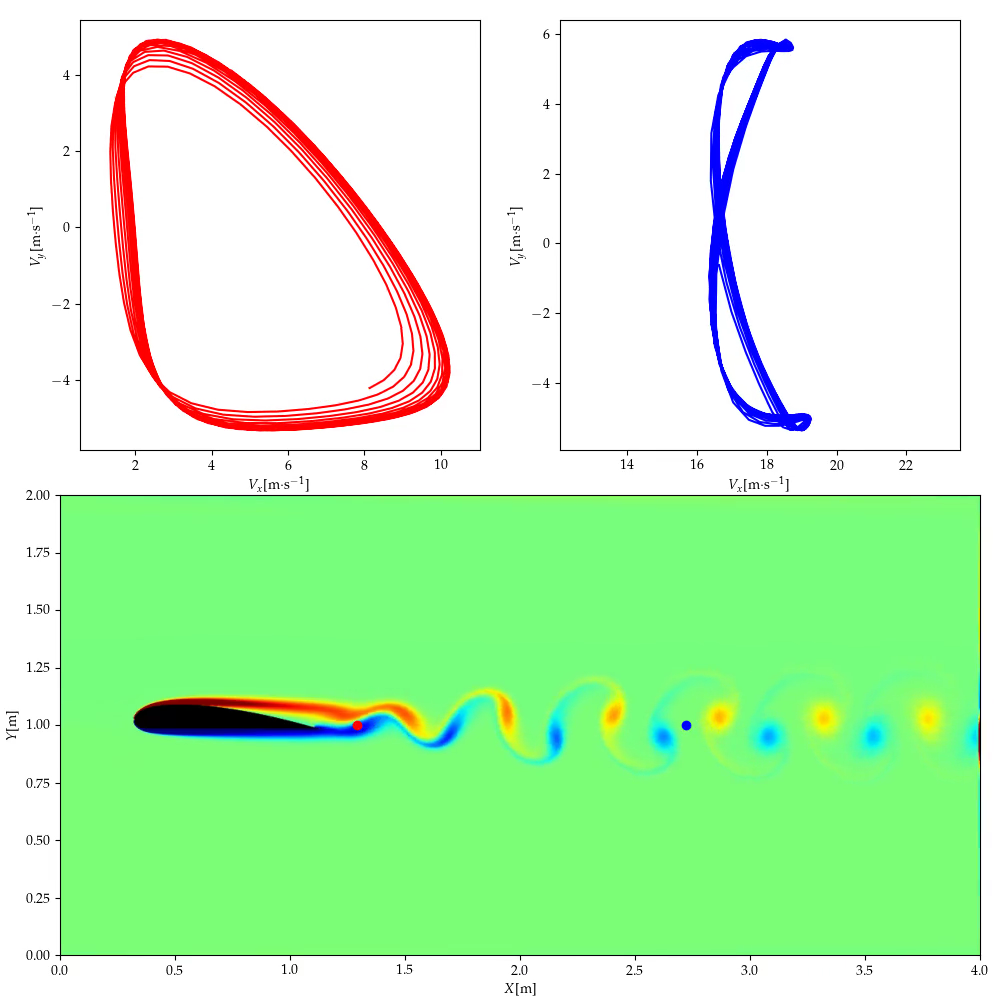
\includegraphics[width=\linewidth]{Fig/VK.png}
  \caption{Allée de Von Karman pour $Re \approx 400$}
  \label{fig:VK}
\end{figure}

Afin d'étudier plus quantitativement nos résultats nous avons choisi deux points d'intérêt au niveau de l'allée de Von Karman et nous avons tracée la trajectoire dans l'espace des phases de ces points, passée un régime de transition, ces trajectoires convergeaient vers une orbite périodique. L'analyse de la trajectoire dans l'espace des phases est un outil
très puissant quand il es question de caractériser les écoulements auquel nous avons à faire.
Très vite lors de nos simulations nous avons systématiquement utilisé le nombre de Reynolds afin de pouvoir avoir une idée avant de lancer la simulation de la physique que nous allions avoir.

